\part{Práctica 3}
\section{Actividad 3-1}
\label{p31}
\begin{center}
    \parbox{12cm}{\justify\textit{Escoja una de las bases de datos de clasificación para el trabajo de las dispuestas en Moodle (Breast Cancer, Dermatology, Fantasmas, Glass, Vehicle, Wine, Zoo). \\
    Se entiende que además de pasarla a formato .arff ya ha aplicado el preprocesamiento necesario en función del fichero ``\textbf{Pistas sobre los datasets con posible preprocesamiento a simple vista.pdf}'', en el caso de que sea una de las bases de datos que lo requiera.
    \begin{itemize}
        \item Aplique el preprocesamiento adicional (si se puede aplicar sobre: 1) reemplazamiento de datos perdidos, 2) normalización y 3) paso de nominal a binario u ordinar a numérico. Explique el preprocesamiento que haya llevado a cabo en los aspectos citados, y de no tener que hacerlo explique también por qué.
    \end{itemize}}}
\end{center}

La base de datos seleccionada (Criaturas de competición Kaggle: dataset371.csv) contiene los siguientes campos:
\begin{itemize}
    \item id: es un identificador único numérico autoincremental.
    \item bone\_length: longitud media del hueso en la criatura, normaliado entre 0 y 1.
    \item rotting\_flesh: Porcentaje de carne podrida en la criatura, normalizado entre 0 y 1.
    \item hair\_length: longitud media del pelo, normalizado entre 0 y 1.
    \item has\_soul: porcentaje de alma en la criatura, entre 0 y 1.
    \item color: color dominante de la criatura, nominal con seis valores posibles.
    \item type: clase asignada, con valores ``Ghost'', ``Goblin'' y ``Ghoul''.
\end{itemize}

El primer paso a simple vista es eliminar el campo id, ya que los valores únicos no nos dan ninguna información acerca de la clase del patrón. No se observan datos perdidos y los atributos numéricos ya se encuentran normalizados. En este caso, los dos algoritmos que se utilizarán posteriormente soportan atributos con valores tanto nominales como numéricos continuos, por lo que no es necesario realizar ninguna discretización o reemplazo por números.

Respecto a la selección de atributos, gracias al filtro \code{CorrelationAttributeEval} podemos ver que el atributo \code{color} tiene muy poca influencia sobre la clase (ver fig. \ref{fig:fantasmas-irrelevantes}) por lo que se procede a su eliminación. También se han estudiado las posibles correlaciones entre los atributos, pero ninguna es significativa (ver fig. \ref{fig:fantasmas-correlaciones}) No se han encontrado valores extremos aunque sí 5 outliers, pero estos no requieren tratamiento.

\begin{figure}[H]
    \centering
    \begin{minipage}{0.5\textwidth}
        \centering
        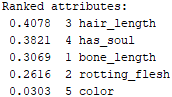
\includegraphics[scale=.9]{preproc-01-irrelevantes-b}
        \caption{Influencia de los atributos en la clase}
        \label{fig:fantasmas-irrelevantes}
    \end{minipage}\hfill
    \begin{minipage}{0.5\textwidth}
        \centering
        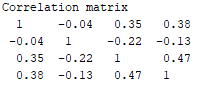
\includegraphics[scale=1]{preproc-02-correlaciones}
        \caption{Matriz de correlaciones entre atributos}
        \label{fig:fantasmas-correlaciones}
    \end{minipage}
\end{figure}


%-------------------------------------------------------------------------------
%-------------------------------------------------------------------------------
%-------------------------------------------------------------------------------
\clearpage
\section{Actividad 3-2}
\label{p32}
\begin{center}
    \parbox{12cm}{\justify\textit{Con la base de datos escogida anteriormente, use el algoritmo de clasificación \textbf{KNN} (IBK en Weka) con un 10-fold crossvalidation. Use un valor de vecinos $k=3$ dejando por defecto el resto de parámetros.
    \begin{itemize}
        \item Interprete la salida en cuanto a los valores de las métricas que proporciona Weka.\\
        Tenga en cuenta si se clasifican bien todas las clases de su problema (TP Rate por clase) y fíjese también en la matriz de confusión. \\
        Para explicar los resultados, haga uso de tablas donde se muestren los valores que está interpretando.
    \end{itemize}}}
\end{center}

Para este ejercicio se ha utilizado la base de datos preprocesada del ejercicio anterior. Se va a ejecutar el algoritmo KNN (llamado IBk en Weka) considerando los 3 vecinos más cercanos. Esto significa que se va a dividir el conjunto de datos en 10 partes, los patrones de cada una de las cuales se clasificará en función de la clase de los 3 vecinos más cercanos del subconjunto complementario. Para determinar los vecinos más cercanos se empleará la distancia euclídea y un algoritmo de búsqueda por fuerza bruta llamado \code{LinearNNSearch} en Weka. La configuración empleada se puede ver en la figura \ref{fig:knn-configuracion}.

\begin{figure}[ht]
    \centering
    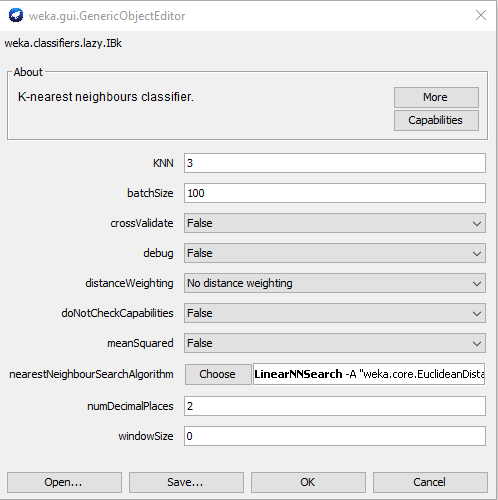
\includegraphics[scale=.7]{knn-01-configuracion}
    \caption{Configuración del clasificador IBk}
    \label{fig:knn-configuracion}
\end{figure}

Podemos ver los resultados que arroja el clasificador en la figura \ref{fig:knn-resultados}. Hay un 70,89\% de patrones bien clasificados (263) frente a un 29,11\% de patrones mal clasificados (108). El valor 0,5631 del estadístico Kappa nos indica que el clasificador está aproximadamente a medio camino entre el azar ($\kappa=0$) y un clasificador perfecto ($\kappa=1$).

Los TP Rates tambien nos indican que el clasificador es mejor que uno al azar, que arrojaría valores de 0,333 (igual para todas las clases). En estos datos podemos observar también que se reconoce peor la clase Goblin, lo que se confirma con el valor de precisión mínima ---que corresponde a esta clase--- y la matriz de confusión, donde podemos ver que sólo 73 de los 125 goblins han sido correctamente clasificados.

\begin{figure}[ht]
    \centering
    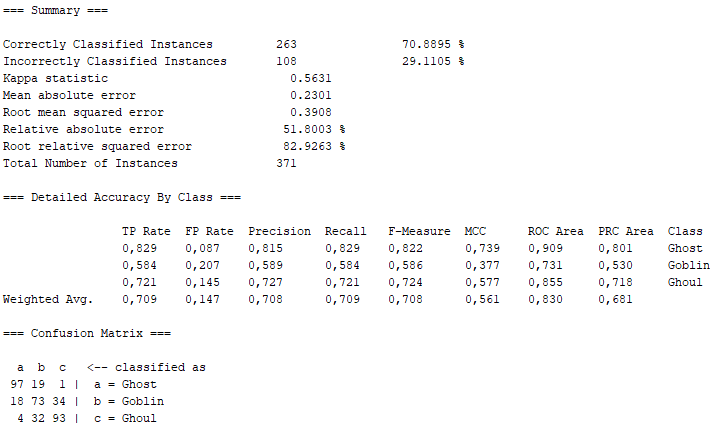
\includegraphics[width=\textwidth]{knn-02-resultado}
    \caption{Resultados del clasificador IBk con un 10-fold}
    \label{fig:knn-resultados}
\end{figure}



%-------------------------------------------------------------------------------
%-------------------------------------------------------------------------------
%-------------------------------------------------------------------------------
\clearpage
\section{Actividad 3-3}
\label{p33}
\begin{center}
    \parbox{12cm}{\justify\textit{Con la base de datos escogida anteriormente, ejecute el algoritmo Simple-Logistic con 10-fold crossvalidation.
    \begin{itemize}
        \item Analice los modelos obtenidos, las variables que podrían ser más influyentes (valores $\beta$) variables que no se usan y métricas. \\
        Use tablas para explicar los resultados de manera que haya una lectura legible.
    \end{itemize}}}
\end{center}

En esta ocasión utilizaremos el clasificador \code{SimpleLogistic}. Un clasificador de tipo logístico funciona aplicando una transformación logística a la suma ponderada de los valores del patrón para cada clase. La diferencia entre Logistic y SimpleLogistic es que Logistic calcula la última clase como el complemento de la suma del resto de clases hasta 1. Se asigna al patrón la clase correspondiente al resultado más alto. En la figura \ref{fig:sl-configuracion} podemos ver el formulario de configuración del clasificador SimpleLogistic de Weka.

\begin{figure}[ht]
    \centering
    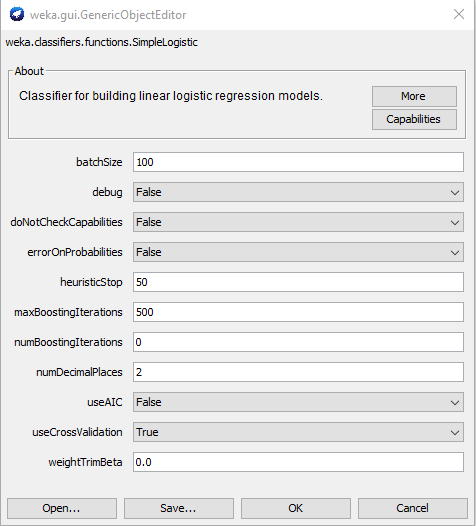
\includegraphics[scale=.7]{sl-01-configuracion}
    \caption{Configuración del clasificador SimpleLogistic}
    \label{fig:sl-configuracion}
\end{figure}

En la figura \ref{fig:fantasmas-logistic-betas} y el cuadro \ref{cuadro:fantasmas-logistic-betas} podemos ver las sumas ponderadas de casa clase, donde los pesos (valores $\beta$) nos dan una idea de la influencia de cada variable independiente en la determinación de la clase. Así podemos ver que para la clase Ghost, los atributos bone\_length, hair\_length y has\_soul influyen muy negativamente mientras que rooting\_flesh lo hace positivamente, justo lo contrario que ocurre en la clase Ghoul. En la clase Goblin vemos que la variable bone\_length no influye, hair\_length y has\_soul lo hacen muy levemente y rooting\_flesh influye negativamente.

\begin{figure}[H]
    \centering
    \begin{minipage}{0.33\textwidth}
        \centering
        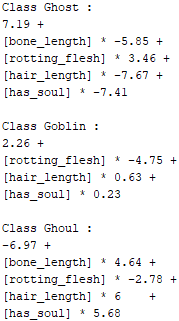
\includegraphics[trim={0cm 5.9cm 0cm 0.08cm},clip]{sl-02-betas}
    \end{minipage}\hfill
    \begin{minipage}{0.33\textwidth}
        \centering
        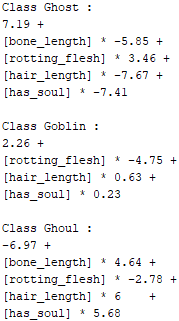
\includegraphics[trim={0cm 2.6cm 0cm 3cm},clip]{sl-02-betas}
    \end{minipage}\hfill
    \begin{minipage}{0.33\textwidth}
        \centering
        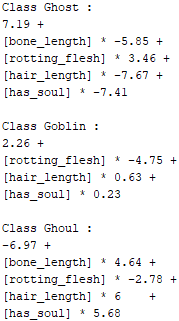
\includegraphics[trim={0cm 0cm 0cm 5.9cm},clip]{sl-02-betas}
    \end{minipage}
    \caption{Pesos de los atributos para cada clase}
    \label{fig:fantasmas-logistic-betas}
\end{figure}

\begin{table}[ht]
    \centering
    \begin{tabular}{|r|r|r|r|r|r|}
    \hline
    \rowcolor[HTML]{9B9B9B} 
    {\color[HTML]{FFFFFF} } & \multicolumn{1}{c|}{\cellcolor[HTML]{9B9B9B}{\color[HTML]{FFFFFF}$\beta_0$}} & \multicolumn{1}{c|}{\cellcolor[HTML]{9B9B9B}{\color[HTML]{FFFFFF} $\beta_1$}} & \multicolumn{1}{c|}{\cellcolor[HTML]{9B9B9B}{\color[HTML]{FFFFFF} $\beta_2$}} & \multicolumn{1}{c|}{\cellcolor[HTML]{9B9B9B}{\color[HTML]{FFFFFF} $\beta_3$}} & \multicolumn{1}{c|}{\cellcolor[HTML]{9B9B9B}{\color[HTML]{FFFFFF} $\beta_4$}} \\
    \rowcolor[HTML]{9B9B9B} 
    \multicolumn{1}{|l|}{\cellcolor[HTML]{9B9B9B}} & \multicolumn{1}{c|}{\cellcolor[HTML]{9B9B9B}{\color[HTML]{FFFFFF} sesgo}} & \multicolumn{1}{l|}{\cellcolor[HTML]{9B9B9B}{\color[HTML]{FFFFFF} bone\_length}} & \multicolumn{1}{l|}{\cellcolor[HTML]{9B9B9B}{\color[HTML]{FFFFFF} rotting\_flesh}} & \multicolumn{1}{l|}{\cellcolor[HTML]{9B9B9B}{\color[HTML]{FFFFFF} hair\_length}} & \multicolumn{1}{l|}{\cellcolor[HTML]{9B9B9B}{\color[HTML]{FFFFFF} has\_soul}} \\ \hline
    \cellcolor[HTML]{9B9B9B}{\color[HTML]{FFFFFF} Ghost} & 7,19 & -5,85 & 3,46 & -7,67 & -7,41 \\ \hline
    \cellcolor[HTML]{9B9B9B}{\color[HTML]{FFFFFF} Goblin} & 2,26 & 0 & -4,75 & 0,63 & 0,23 \\ \hline
    \cellcolor[HTML]{9B9B9B}{\color[HTML]{FFFFFF} Ghoul} & -6,97 & 4,64 & -2,78 & 6 & 5,68 \\ \hline
    \end{tabular}
    \caption{Pesos de los atributos para cada clase}
    \label{cuadro:fantasmas-logistic-betas}
\end{table}

Los resultados del clasificador logístico (fig. \ref{fig:sl-resultados}) son sólo ligeramente mejores que los del clasificador KNN del ejercicio anterior. Vemos que hay 9 patrones correctamente clasificados más que en el anterior, lo que lleva a un $CCR=73,32\%$. En línea con esto, tenemos también un índice Kappa superior: $\kappa=0,5996$.

Por su parte, los TP Rates nos indican que, mientras que ha mejorado el reconocimiento de patrones de clase Ghost y Ghoul, ha empeorado el reconocimiento de patrones Goblin, que ya era la que peor clasificaba. Esto se refuerza con el descenso de la sensibilidad mínima a 0,536 y la bajada a 67 goblins bien clasificados de 125.

\begin{figure}[ht]
    \centering
    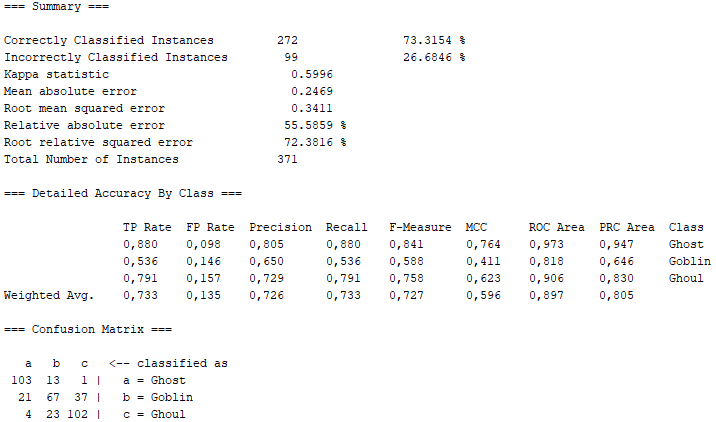
\includegraphics[width=\textwidth]{sl-03-resultado}
    \caption{Resultados del clasificador SimpleLogistic con un 10-fold}
    \label{fig:sl-resultados}
\end{figure}